\chapter{Time metrology}
Aim of this chapter is to present an issue that will be dealt with in this work.
First a concept of theoretical clock will be presented alongside mathematical tools required
for it description and behavior modelling.
This is followed by a more detailed description of stability analysis which is most prominent
field of science dealing with clock behavior.
After describing theoretical clock models an attention will be given to physical implementation
of clock system with special focus on types of clocks used aboard GPS satellites.
Finally current state of the art in GPS clock bias prediction will be presented.
Intention of writing this chapter was that despite clock modelling and frequency analysis being
well known field readers with computer science might not be familiar with it.
For those well versed in frequency analysis most of this chapter can be safely skipped with 
exception of last section that focuses on state of the art in GPS clock prediction as it 
deals with issues that are more specific do described in this work.
It is important to understand that this chapter do not provide comprehensive knowledge about
described field as due to methodology used in presented work that knowledge it is not required.
For more information about clock modelling and stability analysis Handbook of Frequency Stability
Analysis is suggested as reading.


%====================================================================================================
\section{Physical clock implementation}
\label{sec:physical_clock}

%----------------------------------------------------------------------------------------------------
\subsection{Introduction to physical clock implementation}
In all modern time measurement applications frequency source must produce electrical, current or
voltage based, signal. This is because most of precise signal processing and recording is done
in form of either analog or digital circuit.
Most basic form of frequency source is a Resistance Inductance Capacitance (RLC) circuit like 
one shown on Figure \ref{fig:rlc_circ}.
\begin{figure}[htb] 
	\label{fig:rlc_circ}
	\centering
	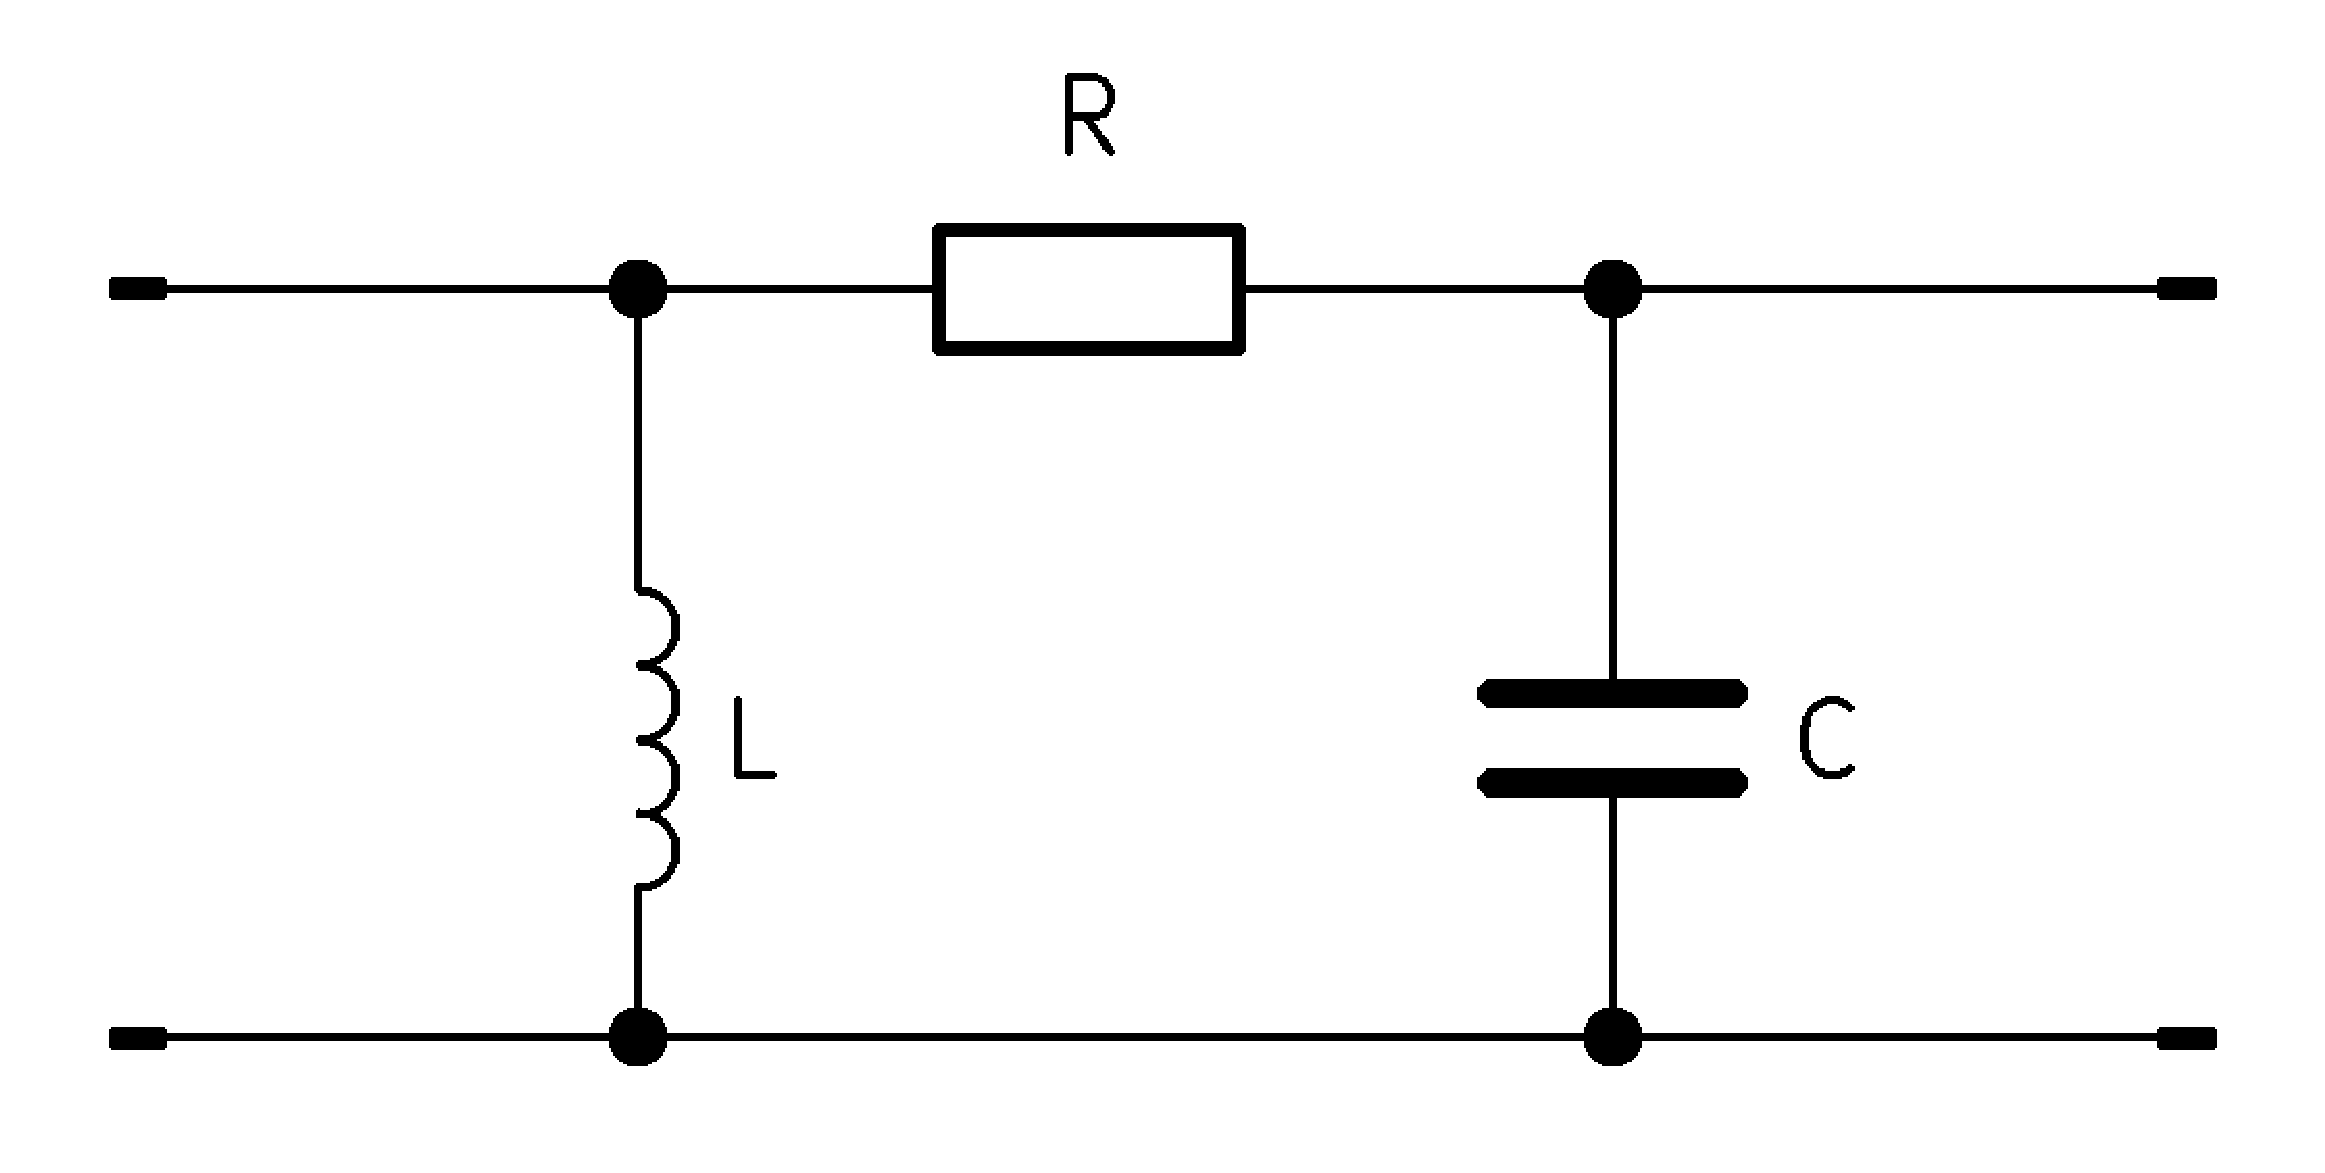
\includegraphics[width=0.5\textwidth]{figures/rlc}
	\caption{RLC circuit example}
\end{figure}
In such circuit electric current is described as a:
\begin{equation}
	\label{equ:rlc_current}
	I = I_{0}sin(\omega t),
\end{equation}
and voltage as a:
\begin{equation}
	\label{equ:rlc_voltage}
	U = U_{0}sin(\omega t + \phi),
\end{equation}
where $I_{0}$ and $U_{0}$ are nominal current and voltage while $\phi$ phase shift of voltage.
This shift depends on values of capacitance, resistance and inductance of circuit in such a way
that:
\begin{equation}
	\label{equ:rlc_freq}
	tg\phi = \frac{\omega L - \frac{1}{\omega C} }{R}.
\end{equation}
Due to a nature of alternating current that results in a impedance of:
\begin{equation}
	\label{equ:rlc_impedance}
	|Z| = \sqrt{R^{2}+ (\omega L - \frac{1}{\omega C})^{2} }.
\end{equation}
As relation between frequency $f$ of signal and its angular speed $\omega$ is described as:
\begin{equation}
	\label{equ:pulse_to_freq}
	\omega = \frac{2\pi}{T} = 2\pi f,
\end{equation}
impedance equation can be rewritten as:
\begin{equation}
	\label{equ:rlc_impedance}
	|Z| = \sqrt{R^{2}+ (2\pi fL - \frac{1}{2\pi f C})^{2} }.
\end{equation}
From equation \ref{equ:rlc_impedance} is seen that resistance influence on impedance is 
constant and independent from frequency. Due to that circuit impedance changes depending on
frequency in relation to capacitance and inductance in such a way that circuit reaches lowest
impedance, and signal highest power, at:
\begin{equation}
	\label{fig:rlc_resonance}
	f_{r} = \frac{1}{2\pi \sqrt{LC}}.
\end{equation}
This means that if a white noise signal will be given on the circuit input on its output 
a frequency equal to resonant frequency $f_{r}$ will be dominant.
\begin{figure}[htb] 
	\label{fig:white_rlc_filter}
	\centering
	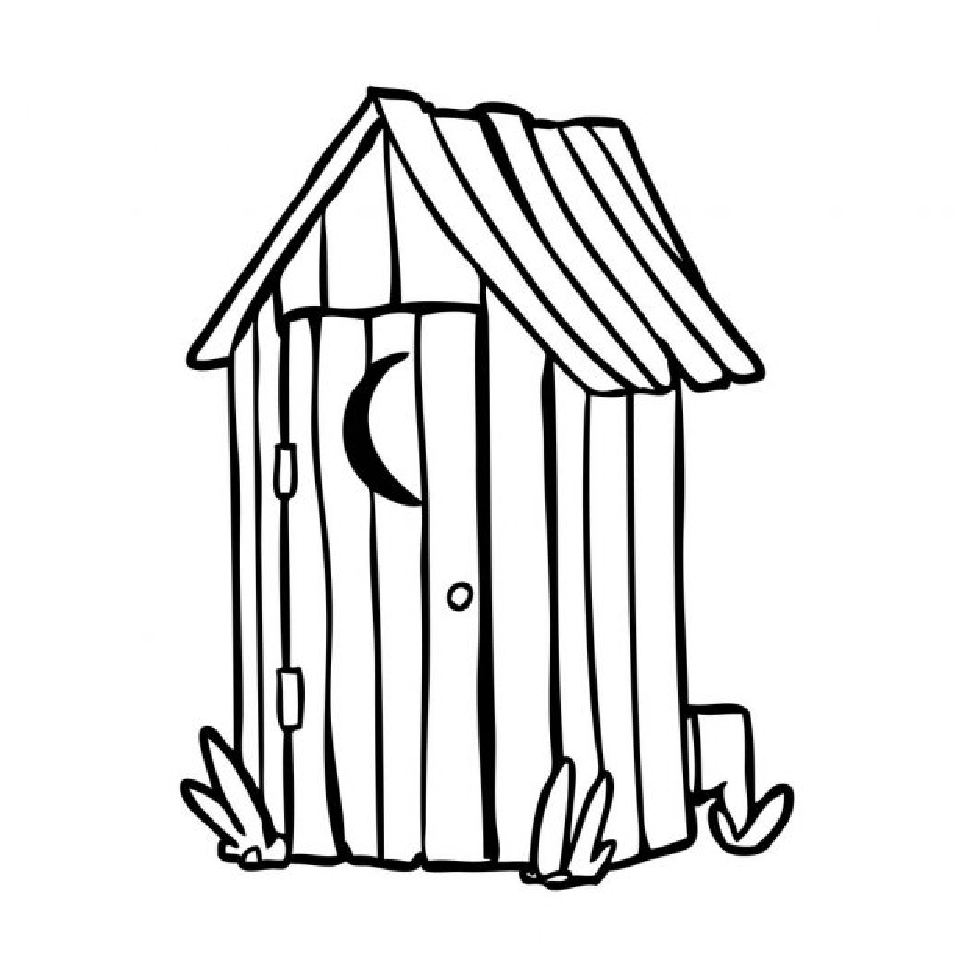
\includegraphics[width=0.5\textwidth]{figures/wychodek}
	\caption{White noise signal before and after RLC circuit}
\end{figure}
While this describes behavior of RLC circuit as a frequency filter another important role of it,
especially in context of this work, is a frequency source.
With assumption that at starting moment $t_{0}$ capacitor is fully loaded and energy stored
in it is described as $Q_{0}$ as well that initial current $I_{0}=0$.
Energy stored in capacitor is released trough resistance as a heat so sum of energies in 
circuit over time can be described as :
\begin{equation}
	\label{equ:circuit_energy}
	\frac{Q^{2}}{2C}+\frac{LI^{2}}{2}+\int_{t_{0}}^{t_{1}}I^{2}R dt = \frac{Q_{0}^{2}}{2C},
\end{equation}
which after derivation over time gives:
\begin{equation}
	\label{equ:circuit_energy_der}
	2\frac{dQ}{dt} + 2I \frac{L\frac{dI}{dt} }{2} + I^{2}R = 0.
\end{equation}
Since electric current is defined as:
\begin{equation}
	\label{equ:current_as_power}
	I = \frac{dQ}{dt},
\end{equation}
equation \ref{equ:circuit_energy_der} can be rewritten as:
\begin{equation}
	\label{equ:circuit_energy_der_mod}
	I(\frac{Q}{C} + L\frac{d^{2}Q}{dt^{2}} + R\frac{dQ}{dt}) = 0.
\end{equation}
As $L>0$ from definition of circuit and for every moment beides initial conditions $I>0$ it is
possible to divide both sides of equation \ref{equ:circuit_energy_der_mod} by $LI$ which will
produce following second-order differential equation:
\begin{equation}
	\label{equ:circuit_energy_der_div}
	\ddot{Q} + \frac{R}{L}\dot{Q} + \frac{1}{LC}Q=0,
\end{equation}
where $\dot{Q}$ is first and $\ddot{Q}$ second derivative of energy over time.
To solve that equation a Laplace transform can be used, in this work details of such process
will not be described and only a resulting solution will be shown:
\begin{equation}
	\label{equ:circuit_energy_solved}
	Q_{t}=Q_{0}e^{-\frac{R}{2L}t}cos(\frac{1}{\sqrt{LC}}t+\phi),
\end{equation}
which means that voltage on capacitor in such circuit can be described as a function of time:
\begin{equation}
	\label{qeu:cap_voltage}
	U_{C}(t) = \frac{Q_c(t)}{C} = U_{0}e^{-\frac{R}{2L}t}cos(\frac{1}{\sqrt{LC}}t+\phi), 
\end{equation}
\begin{figure}[htb] 
	\label{fig:rlc_voltage}
	\centering
	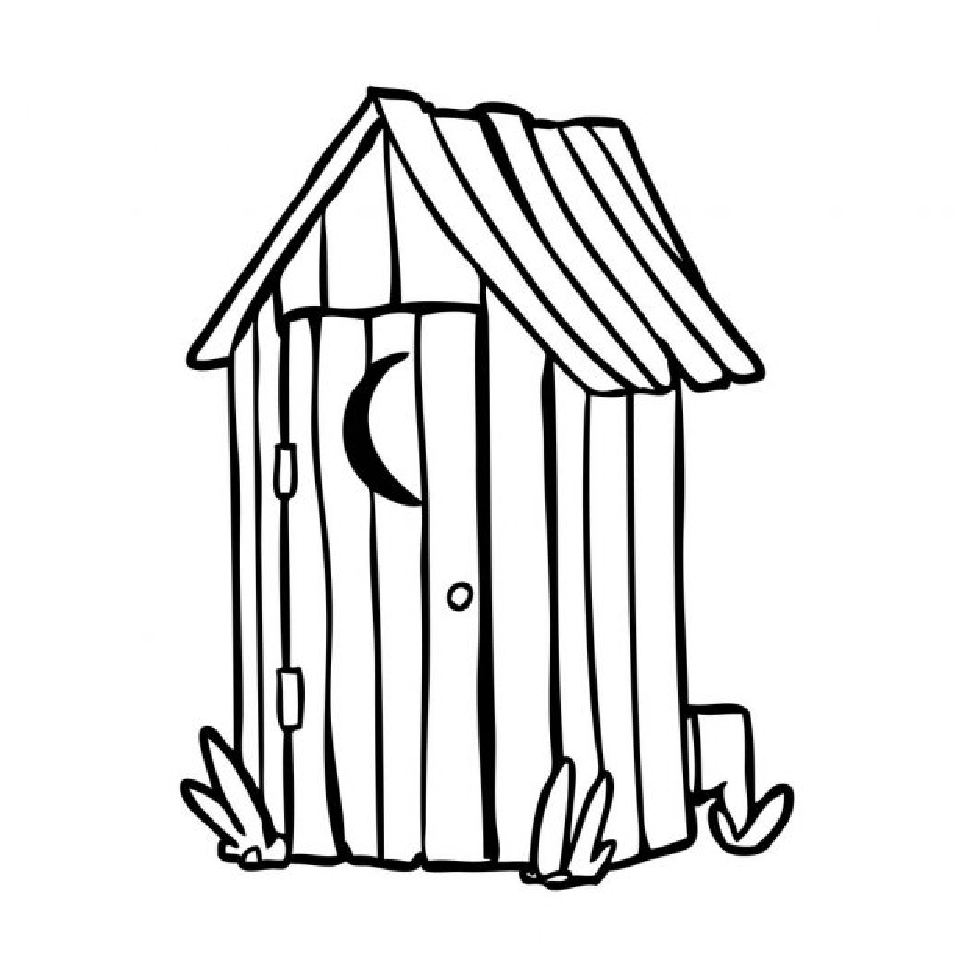
\includegraphics[width=0.5\textwidth]{figures/wychodek}
	\caption{Voltage on RLC circuit capacitor over time}
\end{figure}
%----------------------------------------------------------------------------------------------------
\subsection{Quartz oscillators}

%----------------------------------------------------------------------------------------------------
\subsection{Principles of atomic clock design}


%====================================================================================================
\section{Mathematical clock model}
\textbf{FIXME: MAKE ALL EQUATIONS USE SAME NOTATION}
In context of pure mathematical modelling a clock is understood as a function that describes
offset between two given values for a specific point in time. One of those values is referred 
to as the reference clock and it is considered to always return correct time $T_{r}(t)=t$.
It is important to understand that in physical systems value of $t$ is not only inaccessible, as
every measurement instrument have some degree of uncertainty, but do not exists at all.
This is due to time dilatation effect, derived from special theory of relativity, that causes
time to flow differently in systems that move with velocities close to speed of the light.
This issue is dealt with by selecting most precise physical clock available as the reference
clock and modelling difference between it and other clocks, including time dilatation effects,
as their bias.
Main goal of modeling clocks is to retrieve a value of $t$, which is equal to $T_{r}(t)$, based
on value read from given clock $T_{c}(t)$. 
As relation between those clock is fully described by analyzed clock bias 
$b_{c}(t)=T_{r}(t)-T_{c}(t)$ clock model is equivalent to just a bias model.

%----------------------------------------------------------------------------------------------------
\subsection{Discrete and continuous clock models}
There are two possible approaches to mathematical clock modelling, one of them is continuous
clock model that relies on differential equation for description of its behavior.
In this approach clock bias is modeled as :
\begin{equation}
	\label{equ:continous_clock}
	b_{c}(t) = T_{r}(t_{0}) +  \int_{t_{0}}^{t} \varepsilon_{c}(\tau) d\tau ,
\end{equation}
where:
\begin{itemize}
	\item $t$ is the independent time argument,
	\item $b_{c}(t)$ is the clock bias at time $t$,
	\item $t_{0}$ is time at which clock was synchronized with reference ($b_{c}(t_{0})=0$),
	\item $T_{r}(t_{0})$ is value of reference clock at $t_{0}$,
	\item $\varepsilon_{c}(\tau)$ is the normalized frequency offset of a clock.
\end{itemize}
The branch of science that deals with continuous clock modelling is called stability analysis.
In this work no more attention will be given to that approach as due to nature of data as well as
choice of prediction algorithms favour a discrete clock model.
In discrete clock model bias is described as :
\begin{equation}
	\label{equ:discrete_clock}
	b_{c}(i) = T_{r}(i) - T_{c}(i),
\end{equation}
where $i \in \mathbb{N}$ is the number of measurement.
One of main differences between continuous and discrete models is that in latter case bias is 
considered only as a difference between two individual measurements where in case of 
continuous model all differences starting from synchronization are taken into account.
Another important change is that in discrete model clock is a function $\mathbb{N} \to \mathbb{R}$
instead of $\mathbb{R} \to \mathbb{R}$ like it was in case of continuous model. 
This requires redefinition of reference clock from $T_r{t}=t$ into:
\begin{equation}
	\label{equ:discrete_reference}
	T_{r}(i) = \Delta T_r i,
\end{equation}
where $\Delta T_r$ is the measurement period of reference clock.
In such model $T_{r}$ as well as $T_{c}$ are time series which means that $b_{c}$ is also one.
This means that methodologies related to time series analysis like \textbf{TODO : LIST METHODS}
can be used.
Usually clocks are modelled as a linear combination of several deterministic and stochastic 
components as shown on Figure \ref{fig:clocks_example}. 
\begin{figure}[htb] 
	\label{fig:clocks_example}
	\centering
	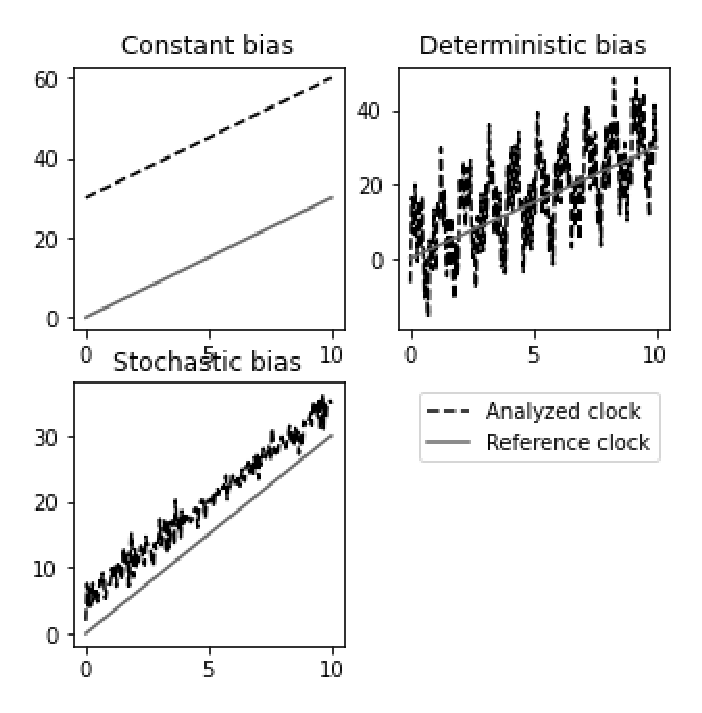
\includegraphics[width=0.5\textwidth]{figures/bias_examples}
	\caption{Example of clock readouts depending of nature of their bias}
\end{figure}
More information on exact clock and noise models will be given in following sections.

%----------------------------------------------------------------------------------------------------
\subsection{Basic clock model}
Basic clock model is a deterministic representation of clock as a second-order linear differential
equation.
\begin{equation}
	\label{equ:basic_clock}
	\ddot{x}(t)=z(t).
\end{equation}
Solution to that equation is
\begin{equation}
	\label{equ:basic_clock_solved}
	x(t)=x_{0}+y_{0}\tau+0.5z_{0}\tau^{2},
\end{equation}
where:
\begin{itemize}
	\item $x(t)$ is clock measurement at time $t$, also called time-offset or bias,
	\item $y(t)$ is fractional frequency offset,
	\item $z(t)$ is fractional frequency drift,
	\item $\tau$ is time difference defined as $\tau = t-t_{0}$.
\end{itemize}
Values $x_{0}$, $y_{0}$, $z_{0}$ refer to initial state of model at $t=t_{0}$.
Because frequency stability of clock degrades over time, as a result of ageing of physical 
components that they consist of, fractional frequency drift is sometimes called clock 
ageing parameter.
In this work $z(t)$ will be also referred to as the linear frequency drift. This terminology
was applied as in case of data used in this research there is a observable deterministic 
first order frequency drift behaviour.

%----------------------------------------------------------------------------------------------------
\subsection{Oscillator noise model}
Basic clock model is limited as it allows only for description of simple deterministic systems 
while real life implementations of clock are complex system with both deterministic and 
stochastic components. 
As described in section \ref{sec:physical_clock} of this chapter central element of every clock,
including atomic clocks, is an oscillator. That is why to create a more complex clock models 
an oscillator noise model must be created.
Role of this model is to derive a clock frequency and phase form an actual physical observation 
which in case of an atomic clock is voltage signal.
Equation describing voltage level on quartz oscillator, which is type of oscillator present in
atomic clocks, can be described by an equation:
\begin{equation}
	\label{equ:quartz_voltage}
	U(t)=(U_{0}+\epsilon(t))sin(2\pi \nu_{0}t + \phi(t)),
\end{equation}
where:
\begin{itemize}
	\item $U_{0}$ is peak voltage amplitude,
	\item $\nu_{0}$ is nominal frequency,
	\item $\phi(t)$ represents random phase deviations,
	\item $\epsilon(t)$ represents random amplitude deviations.
\end{itemize}
Since variation in signal amplitude do not influence measurements of signal frequency, save for
extreme cases where it drops so low that signal peak is not registered, it can be ignored in 
equation used for frequency stability analysis.
This means that equation actually used is:
\begin{equation}
	\label{equ:quartz_voltage_simplified}
	U(t)=U_{0}sin(2\pi \nu_{0}t + \phi(t)).
\end{equation}
Instantaneous clock frequency can be defined as the time derivative of the phase as demonstrated
on following equation:
\begin{equation}
	\label{equ:inst_frequency}
	\nu(t) = \nu_{0}+ \frac{1}{2\pi} \frac{d\phi}{dt},
\end{equation}
where $\frac{d\phi}{dt}$ represents instantaneous frequency offset.
The performance of the clock oscillator is determined by the frequency stability and not 
total frequency and the value of frequency offset is usually small in relation to measured.
Because of that it is more meaningful to describe clock stability with normalized, or fractional,
frequency as described in equation:
\begin{equation}
	\label{equ:normalized_frequency}
	y(t) = \frac{\nu(t)-\nu_{0}}{\nu_{0}} = \frac{dx}{dt}
\end{equation}
where
\begin{equation}
	\label{equ:what_is_time_offset}
	x(t) = \frac{\phi(t)}{2\pi \nu_{0}}
\end{equation}
is bias described in the units of time.


%----------------------------------------------------------------------------------------------------
\subsection{Standard clock model}
Standard clock model is most commonly used mathematical description of the clock that models it as
driven by an oscillator that is in periodic motion around a nominal frequency.
It models how precise clocks are subject to both deterministic bias as well as stochastic 
frequency fluctuations.
Mathematically the standard clock model is represented as a first order stochastic differential
equation . Two state model, with states representing time offset and fractional frequency offset
is described by Galleani. However in this work more focus will be given to three state model 
with states representing clock bias, fractional frequency offset and frequency drift.
This model was presented by Chaffee in 1987 and is described as :
\begin{equation}
	\label{equ:three_state_clock}
	\left[ \begin{array}{c} dx(t)\\ dy(t)\\ dz(t) \end{array} \right] =
	\left[ \begin{array}{ccc} 0& 1& 0\\ 0& 0& 1\\ 0& 0& 0 \end{array} \right]
	\left[ \begin{array}{c} x(t)\\ y(t)\\ z(t) \end{array} \right] dt +
	\left[ \begin{array}{c} d\epsilon(t)\\ d\zeta(t)\\ d\eta(t) \end{array} \right] 
\end{equation}
which is using matrix notation can be described as :
\begin{equation}
	\label{equ:clock_matrix}
	dX(t) = AX(t) +dB(t).
\end{equation}
In those equations $x(t)$, $y(t)$ and $z(t)$ are respectively clock bias, fractional frequency and
fractional frequency drift while $\epsilon(t)$ $\zeta(t)$ and $\eta(t)$ are zero mean Gaussian
white noise processes. They are described as:
\begin{itemize}
	\item $\epsilon(t)$ is white frequency modulation (WFM),
	\item $\zeta(t)$ is random walk frequency modulation (RWFM),
	\item $\eta(t)$ is random run frequency modulation (RRFM).
\end{itemize}
With this it is clear that in matrix notation $X$ is clock state matrix, $A$ is state transition
matrix while $B$ is random noise matrix.
As this work do not focuses on stochastic differential equations only a solution for the equation
\ref{equ:three_state_clock} will be shown, for those more interested in how it was calculated 
more basic literature on topic of SDE is suggested.
\begin{equation}
	\label{equ:clock_solved}
	X(t) = \Phi(t,t_{0})X(t_{0}) + \int^{t}_{t_0}\Phi(t,\tau)dB(\tau),
\end{equation}
where
\begin{equation}
	\label{equ:what_is_phi}
	\Phi(t,t_{0}) = e^{At-t_{0}} = \sum^{\infty}_{0}\frac{(A(t-t_{0}))^2}{n!},
\end{equation}
and $X_{0}$ is the initial condition.
If $X(t_{0})$ is assumed to be a non-random constant then $X(t)$ is a Gaussian process with 
stationary increments and clock bias at time $t$ can be calculated with equation:
\begin{equation}
	\label{equ:bias_final}
	x(t)=x(t_{0}) + y(t-t_{0}) + z(t_{0})\frac{(t-t_{0})^2}{2} + \int^{t}_{t_{0}}d\epsilon(\lambda)
	+ \int^{t}_{t_{0}}(t-\lambda)d\zeta(\lambda) 
	+ \int^{t}_{t_{0}}\frac{(t-\lambda)^2}{2}d\eta(\lambda),
\end{equation}
where the integrals represent noise processes and terms above 2 are excluded.

%====================================================================================================
\section{Stability analysis}
Quality of an oscillator is determined by its frequency stability over time. 
As both phase and frequency influence clock readouts so stability analysis must focus on both.


%----------------------------------------------------------------------------------------------------
\subsection{Allan variance}
Allan variance, also know as the two-sample variance, is the default descriptive statistic
for time and frequency measurements.
This is because standard variance is not suitable for modelling non stationary processes.
The Allan variance is formally adopted as a standard for characterising and reporting instabilities
in phase, frequency or amplitude measurements in time domain.
Allan variance is an infinite time average of the square of the difference of two fractional
frequency measurements:
\begin{equation}
	\label{equ:allan_first}
	\sigma^{2}_{y}(\tau)=0.5\langle (\hat{y}_{k+1}-\hat{y}_k)^{2}  \rangle,
\end{equation}
where $\langle \rangle$ denotes the infinite time average operator while $\hat{y}_k$ is a 
frequency at time $t_{k}$. Hat over variable indicates that value is estimated from phase
measurements with following equation:
\begin{equation}
	\label{equ:y_hat}
	\hat{y}_{k}=\frac{1}{\tau}\int^{t_{k+1}}_{t_{k}}y(t)dt =
	\frac{x(t_{k+1})-x(t_{k})}{\tau},
\end{equation}
In real world application Allan variance is calculated basing on the set of a measurements which
is always a finite set. Therefore as data worked upon is finite and discrete in time domain 
Allan variance can be described as:
\begin{equation}
	\label{equ:allan_discrete}
	\sigma^{2}_{y}(\tau) = \frac{1}{2(M-1)}\sum^{M-1}_{k=1}(\hat{y}_{k+1}-\hat{y}_{k})^2,
\end{equation}
where $M$ denotes number of measurements.
By substituting selected values in equation \ref{equ:allan_discrete} Allan variance can be
described as a function of phase or time offset
\begin{equation}
	\label{equ:allan_discrete2}
	\sigma^{2}_{y}(\tau) = \frac{1}{2(M-1)\tau^{2}}\sum^{M-1}_{k=1}(x_{k+2}-2x_{k+1}+x_{k})^2.
\end{equation}
Even better estimation of Allan variance can be achieved by calculating what it is called a
overlapping Allan variance. This is because it forms all possible overlapping combinations of
available data
\begin{equation}
	\label{equ:overlapping_allan}
	\sigma^{2}_{y}(\tau) = \frac{1}{2(N-2m)\tau^{2}}\sum^{N-2m}_{k=1}(x_{k+2m}+2x_{k+m}+x_{k})^2.
\end{equation}
As overlapping Allan variance provides better results than its basic version in most cases 
literature dealing with stability analysis will use term Allan variance to refer to it 
overlapping version unless specified otherwise.
There is also one more variant called modified Allan variance that unlike all previous examples
can distinguish between WPM and FPM.
In term of phase modified Allan variance is described as:
\begin{equation}
	\label{equ:modified_allan}
	\sigma^{2}_{y}(\tau)=\frac{1}{2m^{2}\tau^{2}(N-3m+1)\tau^{2}}\sum^{N-3m+1}_{j=1}(
	\sum^{j+m-1}_{k=j}(x_{k+2m}-3x_{k+m}+x_{k})^2)
\end{equation}

%--------------------------------------------------------------------------------------------------
\subsection{Hadamard variance}
Hadamard variance was derived from the Hadamard transform for use in stability analysis by 
Baugh.  As the Allan variance describes a second-order phase variation so Hadamard variance 
describes third-order phase variation.
Unlike Allan variance Hadamard variance is insensitive to linear frequency drift, this is 
especially important in context of this work as rubidium clocks used in GPS satellites have a 
prominent linear drift.
As with Allan variance the overlapping version of equation is used as default:
\begin{equation}
	\label{equ:overlapping_hadamard}
	\sigma^{2}_{H} = \frac{1}{6(N-3m)\tau^2}
	\sum^{N-3m}_{k=1}(x_{k+3m}-3x_{k+2m}+3x_{k+m}-x+{k})^{2}
\end{equation}

%====================================================================================================
\section{Modeling noise}
Noise process is defined as a stochastic time varying phenomenon that at each moment in time is
represented by a random variable $X(t)$ whose probability density function is denoted as $f_{X}(t)$.
Such process can be either continuous or discrete depending on model that is worked on, in case 
of real life application $f_{X}(t)$ may not be known.
In context of time and frequency metrology such signal components are modelled as a power-law
noise processes. This is special type of noise process whose frequency and phase noise power 
spectral densities vary as as a power of the Fourier frequency.
Power noise process can be described in relation to frequency fluctuations as:
\begin{equation}
	\label{equ:power_noise_freq}
	S_{y}(f) \propto f^{\alpha},
\end{equation}
where $S_{y}(f)$ denotes fluctuations of frequency $f$ and $\alpha$ describes a power-law of
frequency noise.
When dealing with time measurements it can be more useful to describe a relation between clock 
bias, also called a phase variation, and noise:
\begin{equation}
	\label{equ:power_noise_phase}
	S_{x}(f)=\frac{S_{y}(f)}{(2\pi f)^2} \propto f^{\beta},
\end{equation}
where $\beta$ is description of power-law phase noise and is calculated as $\beta=\alpha-2$.
Power-law noise can also be described in time domain in relation to Allan variance.
In this form process is described as :
\begin{equation}
	\label{equ:power_noise_time}
	\sigma^{2}_{y}(\tau)=g_{\gamma}\tau^{\gamma}
\end{equation}

----------------------------------------------------------------------------------------------------
\subsection{Oscillator noise as linear combination of power-law noises}
In general there are five distinct power-law processes, white phase modulation (WPM), flicker 
phase modulation (FPM), white frequency modulation (WFM), flicker frequency modulation (FFM) and
random walk frequency modulation (RWFM).
All of them can be described by parameters $\alpha$, $\beta$, $\gamma$
\begin{table}[htb] 
	\centering
	\caption{Parameters of power-law noise variants}
	\label{tab:power-noise}
	\begin{tabular}{lccc}
		\hline
		\hline
		Noise type& $\alpha$& $\beta$& $\gamma$\\
		\hline
		WPM&   2 &  0& -3\\
		FPM&   1 & -1& -2\\
		WFM&   0 & -2& -1\\
		FFM&  -1 & -3& -0\\
		RWFM& -2 & -4&  1\\
		\hline
		\hline
	\end{tabular}
\end{table}
The power spectral density of oscillator noise is described as a linear combination of 
those power noise processes:
\begin{equation}
	\label{equ:linear_noise_comb}
	S_{y} = \sum_{\alpha=-2}^{2}h_{\alpha}f^{\alpha},
\end{equation}
where $h_{\alpha}$ indicates influence of a specific noise type on overall oscillator noise.
For general time representation a modified Allan variance can be used:
\begin{equation}
	\label{equ:allan_noise_comb}
	\sigma^{2}_{y} = \sum_{\gamma=-3}^{1}g_{\gamma}\tau^{\gamma},
\end{equation}
where $\tau$ is analysis interval.
%----------------------------------------------------------------------------------------------------
\subsection{White phase modulation noise}
White phase modulation noise is a constant-mean, constant-variance stochastic process.
Discrete white phase modulation noise is represented by a sequence of independent random variables
with identical Gaussian probability density functions which are denoted as  
$\mathcal{N}(\mu,\sigma^{2})$
\begin{figure}[htb] 
	\label{fig:wpm}
	\centering
	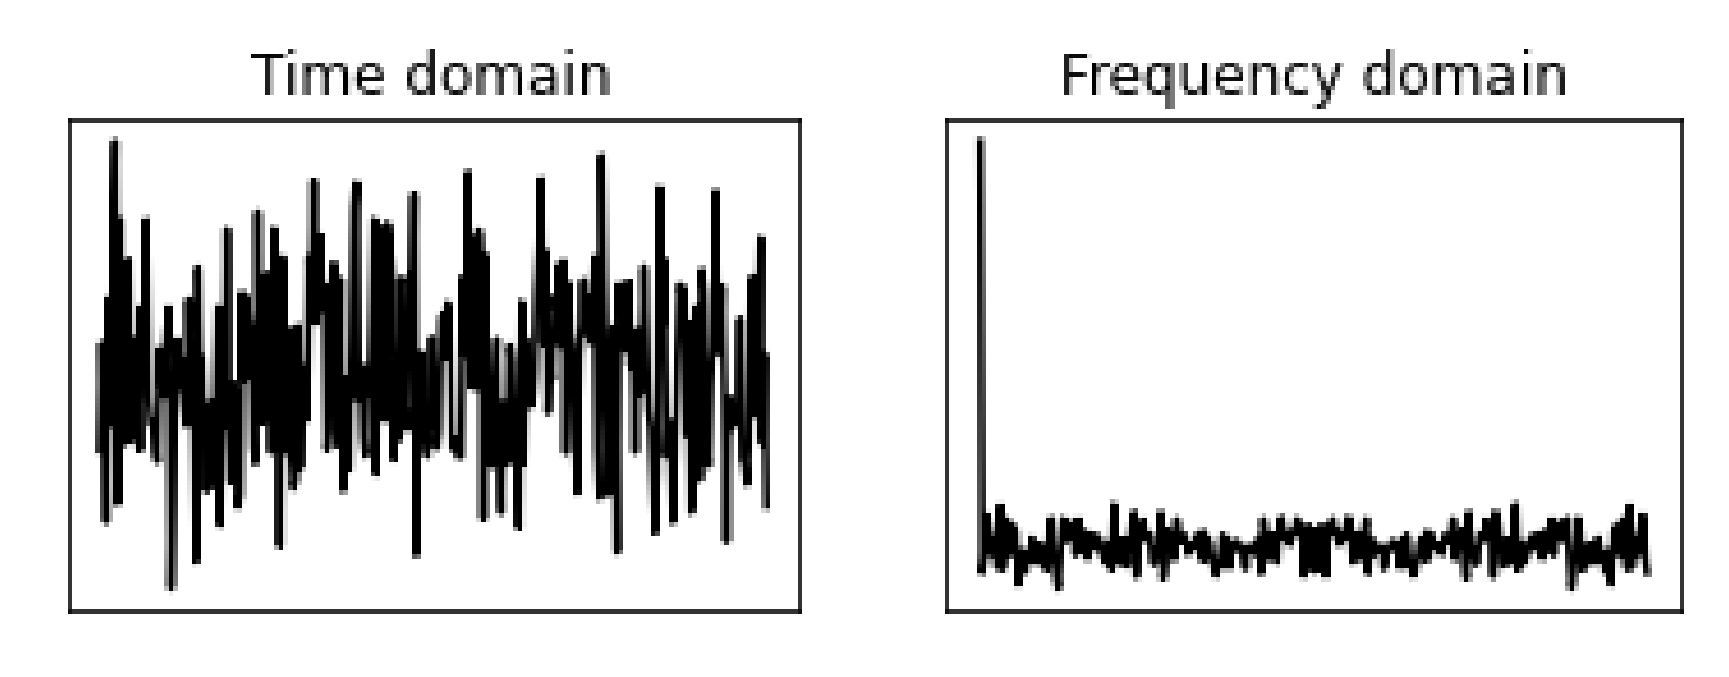
\includegraphics[width=0.7\textwidth]{figures/wpm}
	\caption{White phase modulation in time and frequency domains}
\end{figure}

%----------------------------------------------------------------------------------------------------
\subsection{Flicker phase modulation noise}


%----------------------------------------------------------------------------------------------------
\subsection{White frequency modulation noise}
White frequency modulation is a zero mean white noise sequence 

%----------------------------------------------------------------------------------------------------
\subsection{Flicker frequency modulation noise}

%----------------------------------------------------------------------------------------------------
\subsection{Random walk frequency modulation noise}




%====================================================================================================
\section{State of the art in GPS clock bias prediction}

%----------------------------------------------------------------------------------------------------
\subsection{Time references in GPS}
For correct implementation of beacon based navigation a spatial and temporal reference frames 
must be agreed upon. In case of GPS information about it can be found in International Earth
Orientation Service Conventions. Due to the scope of this work attention will be given only to
standards related to time measurements. The first temporal reference that have to be introduced
is Geocentric Coordinated Time (TCG). It is a timescale that is defined to be consistent with
general relativity theory in proximity of the non-rotating Earth. Due to that TCG can not be
directly observed an as such is used only as a theoretical standard of timescale.
Next step is definition of still theoretical but physically realizable Terrestrial Time (TT).
Relation between TCG and TT is described as:
\begin{equation}
	\label{equ:tcg_to_tt}
	\frac{dTT}{dTCG} = 1 - \frac{W_{0}}{c^2},
\end{equation}
where $W_{0} = 62636857 m^{2}/s^{2}$ is the Earths gravitational potential at sea level.
This theoretical concept is realised as the International Atomic Time (TAI) which is an
atomic timescale relying on ensemble of frequency sources placed at multiple locations around 
the globe. Base of time measurement for TAI is the SI second which is defined as 
\textit{
	duration of 9 192 631 770 periods of the radiation corresponding to the transition between
	two hyperfine levels of the ground state of the cesium 133 atom, with the cesium atom at 
	rest on the rotating geoid at a temperature of 0 K.
}
TAI is used as a frequency standard for Coordinated Universal Time (UTC) which is the most
commonly used time reference frame in civilian purposes.
In case of GNSS applications TAI is not accessible in real time, therefore a realisation of 
TT dedicated to GNSS must be realised.
For GPS, the World Geodetic System 1984 (WGS84) is adopted with relevant timescales being 
GPS System Time (GPST) ant the realisation of UTC at the United States Naval Observatory 
(UTC(USNO)). GPST is the reference timescale for all GPS devices, both satellites and ground
recievers. Main difference between GPST and UTC is that GPST is a continuous timescale while 
UTC introduces concept of leap seconds.
Relationship between GPST and TAI can be described as:
\begin{equation}
	\label{equ:gpst_to_tai}
	T_{TAI}-T_{GPST} = 19 + X_{USNO},
\end{equation}
where $X_{USNO}$ is bias of US Naval Observatory clock in relation to TAI such that 
$|X_{USNO}| \le 1\mu s$. Value of $19$ seconds is added as zero epoch of GPST is set on 
6 January 1980 and is 19 seconds ahead of TAI zero epoch.

%----------------------------------------------------------------------------------------------------
\subsection{Satellite broadcast polynomial}

%----------------------------------------------------------------------------------------------------
\subsection{IGU products}
The most widely used source of precise clock corrections are products provided 
by International GNSS Service (IGS) \cite{Kouba2009}.
\begin{table}[htb] 
	\centering
	\caption{Variants of IGS products}
	\label{tab:igs_products}
	\begin{tabular*}{\textwidth}{*{5}{l}}
		\hline
		\hline
		Type& Accuracy& Latency& Update& Sample \\
		&&&&interval\\
		\hline
		Broadcaster & 5ns & real time & -- & daily  \\
		Ultra rapid -- predicted & 3ns & real time & at 03, 09, 15, 21 UTC & 15 min  \\
		Ultra rapid -- observed & 150ps & 3-9 hours & at 03, 09, 15, 21 UTC & 15 min  \\
		Rapid & 75ps & 17-41 hours & at 17 UTC daily & 5 min \\
		Final & 75ps & 12-18 days & every Thursday & 30 s \\
		\hline
		\hline
	\end{tabular*}
\end{table}
Values shown in Table \ref{tab:igs_products} refer to satellite clock bias only,  IGS products
provide other information which full description  is available at online repository. 
IGS products can be easily divided into two categories:
\begin{itemize}
	\item real time consisting of transmitted and ultra rapid predicted half,
	\item high latency consisting of ultra rapid observed half as well as rapid and final products.
\end{itemize}
Solutions that have high latency are not usable in real-time navigation and as such will not be
considered in this work. Ultra-rapid observed will be used as a source of
reference time so that if a bias prediction error is equal to zero it means that is
the same as provided by ultra-rapid observed.
As can be seen in Table \ref{tab:igs_products} all real-time solutions provide precision 
at a range of nanoseconds, aim of this work is to show that LSTM networks can provide 
better results than those solutions while still working at real-time response latency.

This work focuses only on GPS satellites which are divided into following blocks:
I, II, IIA, IIR ,IIR-M ,IIF, III.
Blocks I and II were fully retired before research described in that paper began and block
III satellites were active for to short time to generate enough data.
That is why those blocks were not used at all, on the other hand single satellite from block
IIA was used in second phase of experiments however it was retired in mean time and a decision
was made to not use it in next experiments and as such it is not listed in final satellite pool.
This results in total of 30 satellite clocks analyzed with almost all of them are equipped 
with Rubidium clock ensemble witch exception of two satellites from generation IIF 
that use Cesium clocks instead.
Each satellite have an assigned space vehicle number (SVN) and pseudo random noise (PRN).
In this work a PRN will be used as a identifier as it is unique for every active satellite, 
although it can be used again after said satellite gets retired, and ranges from 1 to 32.
Association between satellite PRN, clock and block is shown in Table \ref{table:prn}
\begin{table}[htb] \label{table:prn}
\parindent0pt
\caption{Bias prediction error in relation to regularization and dropout level}
\centering
\begin{tabular}{ l  c  c }
  \hline
  \hline
  Generation& clock type& satellites\\  \hline
  IIA & Rb& 18\\  
  IIR & Rb& 2 11 13 14 16 19 20 21 22 23 28\\ 
  IIR-M & Rb& 5 7 12 15 17 29\\ 
  IIF & Rb& 1 3 6 9 10 25 26 27 30 32\\ 
  IIF & Cs& 8 24 \\ \hline \hline
 \end{tabular}
\end{table}
For satellites with rubidium based clock ensembles bias have a very distinct constant drift
that makes data appear linear, it can be seen for satellites 01 and 08. 
On the other hand in case of cesium based clock ensembles for which constant drift is much 
smaller other sources of bias are visible, like seen for satellite 24.
There is also a single satellite for which, during observed period, constant drift was almost
not present. This was satellite 14 and while no official source of information describes this 
behaviour

